%%%%%%%%%%%%%%%%%%%%%%%%%%%%%%%%%%%%%%%%%%%%%%%%%%%%%%%%%%%%%%%%%%%%%%%%
%
% File  : clib.tex
%
% Author: Stephan Schulz
%
% Contents
% 
%   Frame for the clib documentation.
% 
% Changes
%
% <1> Thu Apr 16 03:18:43 MET DST 1998
%     Added this comment header ;-)
%
%%%%%%%%%%%%%%%%%%%%%%%%%%%%%%%%%%%%%%%%%%%%%%%%%%%%%%%%%%%%%%%%%%%%%%%%


\documentclass{article}

\usepackage{epsfig}

\newcommand \fundoc[2]
{\begin{par}
\vspace*{1ex}\noindent
\texttt{#1}\nopagebreak[4]
\begin{quote}%
#2%
\end{quote}%
\end{par}%
}

\author{Stephan Schulz}
\title{The CLIB hierarchy of libraries\\for\\theorem proving
  tasks\\{\small --very preliminary version--}}

\begin{document}

\maketitle{}

\tableofcontents{}


\section{Introduction}
\label{sec:intro}

CLIB is a layered set of libraries implementing successively more
specialized data types and operations for the construction of theorem
provers and related programs (proof transformation and presentation
tools, learning algorithms, lemma generators and filters, \ldots).
It's current aim is to offer a solid and general base to implement the
\emph{E Equational Theorem Prover} and its environment. However, many
of the lower layers are of general interest. The following modules are
currently implemented:

\begin{description}
\item[BASICS:] This base library offers simple services used by most
  higher levels directly: Error handling and reporting, memory
  management, dynamic strings, as well as indices (based on AVL trees)
  and stacks for some standard data types.
\item[INOUT:] The I/O part of the library offers a standard interface
  to option processing (comparable to the GNU getopt library), a
  powerful and simple to use scanner, and parsing for non-elementary
  build-in data types. 
\item[TERMS:] The terms library is one of the largest and most central
  parts of the library. It implements a shared term term
  representation and elementary operations (create, delete, rewrite,
  match, unify) dealing with terms and substitutions.
\item[ORDERINGS:] This library implements \emph{reduction orderings}
  and related data types on terms.
\item[CLAUSES:] On the next higher level, this layer offers equations,
  literals, clauses and sets of clauses, and the basic inference rules
  for a completion- or superposition-based prover. At this level the
  code starts to get pretty specific to the E project.
\item[HEURISTICS:] The heuristics layer of the library is still under
  serious construction. It offers a lot of general functions for
  analyzing proof problems, but also has very specific stuff for
  controling the search of a given prover.
\item[CONTROL:] This currently last library layer contains the top
  level control functions for the proof process of E.
\end{description}

Even the lower, more general layers of the library make certain
assumptions about the applications. In particular, it is assumed that
programs are not used interactively, and that all errors cause the
program to terminate by calling one of two error functions.

%%% Local Variables: 
%%% mode: latex
%%% TeX-master: "clib"
%%% End: 


\section{Installation and Getting Started}
\label{sec:install_start}

This section should help you to do the first step with the CLIB
library. If you can read this documentation from your own
distribution, you probably can skip it\ldots

\subsection{Installation}
\label{sec:install_start:install}

Installation of the CLIB library should be a very simple step. Once
you have obtained the distribution file \texttt{CLIB.tgz}, you just
need to unpack the distribution, using either GNU \texttt{tar} or the
combination of \texttt{gzip} and a conventional UNIX
\texttt{tar}. This will create a subdirectory named \texttt{CLIB} in
the current directory. To install CLIB now just type 

\begin{verbatim}
cd CLIB
make install
\end{verbatim}
and the library should install itself. If you do not have a recent
version of the GCC compiler, you may need to edit
\texttt{CLIB/Makefile.vars} to select a different compiler and linker, and
to select appropriate options. You may also want to edit this file if
you have a non-standard system and lack the utilities necessary for
the normal building of the library.

The default installation procedure will not build the documentation,
as local \LaTeX{} setups seem to differ a lot between sites. To
build the documentation, you need \LaTeX2e{}. If your local \LaTeX2e{}
executable is named \texttt{latex}, just use

\begin{verbatim}
make documentation
\end{verbatim}
in the \texttt{CLIB} directory to typeset the documentation.
Otherwise, edit the file \texttt{CLIB/Makefile.vars} to point to your
\LaTeX2e{} executable (or \texttt{cd} to \texttt{CLIB/DOC/} and run
\LaTeX2e{} on \texttt{clib.tex} and \texttt{eprover.tex} manually).

\subsection{Getting Started}
\label{sec:install_start:start}

Once you managed to install the library, you may want to look around
and see what is offered. Fig~\ref{fig:install_start:start:structure}
shows the basic layout of the directory structure of CLIB.


\begin{figure}[htb]
  \begin{center}
    \mbox{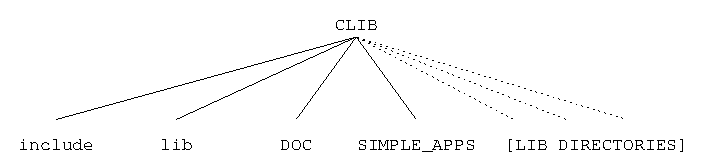
\epsfig{file=file_layout.eps}} % Export with 80%
    \caption{Directory structure of CLIB}
    \label{fig:install_start:start:structure}
  \end{center}
\end{figure}

If the documentation were anywhere close to complete, the \texttt{DOC}
directory would be the most important one for each new user. Even
though this is not yet the case, it should pay to check this directory
and read whatever rudimentary documentation can be found in the file
\texttt{clib.dvi}\footnote{As this text is contained in the CLIB
  documentation, you probably already are reading it\ldots}.

Other important directories are the \texttt{include} directory, which
should contain links to all header files provided by the library, and
the \texttt{lib} directory, which contains the individual library
parts. 

If you want to make use of this library for you own project, the
\texttt{SIMPLE\_APPS} directory has some simple examples that
illustrate the use of the library.

If you change part of the library, and want to remake all modules
depending on your changes, issuing

\begin{verbatim}
make top
\end{verbatim}
in any of the CLIB subdirectories will recompile all parts of the
libraries (more exactly, it will remake all code in directories
specified in the top level \texttt{Makefile} variable
\texttt{CODE}). A simple 

\begin{verbatim}
make
\end{verbatim}
will just remake all parts in the current directory.


\subsection{Conventions used in the Manual}
\label{sec:install_start:conventions}

Each important subsection of the library is first discussed in general
terms, sometimes including the most important data structures. After
that, the relevant functions of the calling interface are described,
giving first the function prototype and then a short description of
the function. Some functionality is implemented by C preprocessor
macros. Such macros are described as though they were functions, but
the prototype given is preceded by \texttt{MACRO}, and arguments may
be given without a type if the macro in question is defined for
multiple types.


%%% Local Variables: 
%%% mode: latex
%%% TeX-master: "clib"
%%% End: 

%%%%%%%%%%%%%%%%%%%%%%%%%%%%%%%%%%%%%%%%%%%%%%%%%%%%%%%%%%%%%%%%%%%%%%%%
%
% File  : basics.tex
%
% Author: Stephan Schulz
%
% Contents
% 
%   Documentation for the BASIC sublibrary of CLIB.
% 
% Changes
%
% <1> Thu Apr 16 03:18:43 MET DST 1998
%     Added this comment header ;-)
%
%%%%%%%%%%%%%%%%%%%%%%%%%%%%%%%%%%%%%%%%%%%%%%%%%%%%%%%%%%%%%%%%%%%%%%%%


\section{Basic Services}
\label{sec:basics}

The BASICS part of the library implements general infrastructure
useful for most programs. This ranges from elementary things like a
\texttt{bool} data type and a NULL pointer to error handling and
memory management.


\subsection{Miscellaneous Stuff}
\label{sec:basics:elementary}


\subsubsection{Usage Information}

\begin{verbatim}
#include <clb_defines.h>

Requires: -
\end{verbatim}

\subsubsection{The \texttt{NULL} Pointer}

\ldots{} is defined as expected. 


\subsubsection{Booleans}

The \texttt{bool} data type can be used in specifications and offers
the two truth values \texttt{true} and \texttt{false} with a twist:
There exist multiple synonyms for both values, to enable the
programmer to put some semantic information into the program code.

The \texttt{bool} data type is currently defined as follows:

\begin{verbatim}
typedef enum
{
   false = 0,
   normal = 0,
   brief = 0,
   true = 1,
   special = 1,
   verbose = 1
}bool;
\end{verbatim}

The C language allows arbitrary values of integer data types
(\texttt{char}, \texttt{int}, \texttt{long} in signed and unsigned
variations, but also all pointer types) as truth values. Only
\texttt{0}\footnote{More exactly, the value that is generated by the
  compiler for the textual string ``\texttt{0}'' in the given type.}
is interpreted as \texttt{false}, all other values are conceptually
equivalent to \texttt{true}. \emph{This means that you cannot compare
  two truth values with \texttt{==} and expect a reasonable result}.
Think about it. \emph{You cannot compare two truth values with
  \texttt{==} and expect a reasonable result}. The various
representations of \texttt{true} are only useful for parameter passing
and variable assignements.


\subsubsection{Generic Integer Types}

The C programming language does not offer truly generic data types.
There are only two ways to manipulate data of more than one type:
Using macros as untyped functions, or using \texttt{void*} pointers as
generic pointers. Both solutions have disadvantages. However, in some
cases the advantages (avoiding the duplication of code) far outweight
the disadvantages of weakening the type concept. For these situations,
CLIB offers a generic data type that can store any pointer value, as
well as \texttt{long} integers (including, of course, values from
subtypes of \texttt{long}). For most implementations of the C
programming language, all of these data types have a 32 bit
representation, and there is no cost for converting between these
types.

The \texttt{IntOrP} data type is defined as a union of a
\texttt{void*} pointer and a \texttt{long} integer:

\begin{verbatim}
typedef union int_or_p
{
   long i_val;
   void *p_val;
}IntOrP;
\end{verbatim}

The two fields have the obvious meaning: Use \texttt{i\_val} to store
numeric values and \texttt{p\_val} for arbitrary pointer types.



\subsubsection{Simple Macros}

For all of these macros, arguments may possibly be evaluated more than
once, i.e. they should probably be free from side effects.

\begin{verbatim}
MACRO MAX(x,y)
MACRO MIN(x,y)
\end{verbatim}
\begin{quote}
  Maximum and minimum of two values for which the \texttt{>} and
  \texttt{<} operators are defined.
\end{quote}

\begin{verbatim}
MACRO ABS(x)
\end{verbatim}
\begin{quote}
  Absolute value of a numerical argument.
\end{quote}

\begin{verbatim}
MACRO XOR(x,y)
\end{verbatim}
\begin{quote}
  \emph{Exclusive or} of two values that are interpreted as truth
  values.
\end{quote}


\subsection{Errors and Runtime Information}
\label{sec:basics:errors}

Programs sometimes need to report special events, e.g. transistion
between different phases or, most importantly, errors during
execution. CLIB distinguishes between \emph{errors}, that always lead
to the termination of the program, \emph{warnings}, which warn the
user about expceptional, but non-critical conditions, and
\emph{verbose messages}, which result from the ordinary execution of
the program.

\subsubsection{Usage Information}

\begin{verbatim}
#include <clb_error.h>
#include <clb_verbose.h>

Requires: lib/BASICS.a
\end{verbatim}


\subsubsection{Errors}

Facilities for error handling fall into two classes: Initialization
routines and global state variables that remain constant after
initialization, and routines and variables that are used only in the
case of error. Initialization of the error handling module is very
simple:

\begin{verbatim}
void         InitError(char* progname)
extern char* ProgName
\end{verbatim}
\begin{quote}
  \texttt{InitError()} stores the name of the program for error
  reporting. The argument has to be a pointer to a constant string
  (giving the name of the program), typically \texttt{argv[0]}. The
  name is available to other parts of the program via the exported
  variable \texttt{ProgName}.
\end{quote}

CLIB always assumes that \emph{errors} are non-recoverable and should
terminate the program. In this case, the program should return an exit
code (via the standard library call \texttt{exit()}) describing the
error condition. Some exit codes are predefined in the enumeration
type \texttt{ErrorCodes}:

\begin{description}
\item[\texttt{NO\_ERROR}:] No error, successful termination of the
  program.
\item[\texttt{OUT\_OF\_MEMORY}:] The program was unable to allocate
  memory. This error will usually be generated by the memory
  management module if a request for memory cannot be satsified.
\item[\texttt{SYNTAX\_ERROR}:] Input to the program does not conform
  to the specification (or rather the implemented parser).
\item[\texttt{USAGE\_ERROR}:] The program was started with incorrect
  options or other arguments.
\item[\texttt{FILE\_ERROR}:] A file operation (usually opening or
  closing) failed.
\item[\texttt{SYS\_ERROR}:] An unspecified system call signalled an
  error.
\end{description}

Reporting an error requires an error code (used as an exit code for
the environment) and an error message for the user. Error messages are
often dynamically generated and include file names or other program
arguments. For simple cases, \texttt{sprintf()} is usually sufficient
to create an error message\footnote{See the \texttt{clb\_dstring}
  module (Sec.~\ref{sec:basics:strings}) for more general, but usually
  less convenient string manipulation functions.}.

\begin{verbatim}
extern char  ErrStr[]
\end{verbatim}
\begin{quote}
  This variable reserves at least \texttt{MAX\_ERRMSG\_LEN} characters
  for creating error messages. This space is always sufficient to
  store any valid UNIX file name and at least
  \texttt{MAX\_ERRMSG\_ADD} additional characters.  You can assume
  that \texttt{MAX\_ERRMSG\_ADD} is large enough for most practical
  considerations.
\end{quote}

\begin{verbatim}
VOLATILE void Error(char* message, ErrorCodes ret)
\end{verbatim}
\begin{quote}
  Print an error message (including the program name and the given
  message) to \texttt{stderr}, and exit the program with the exit code
  \texttt{ret}.
\end{quote}

Failing UNIX system calls or C library calls usually give some
indication about the reason why they failed in the global varible
\texttt{errno} (declared in the standard header file
\texttt{<errno.h>}). If you want to pass on this information to the
user, you should save this value in the CLIB global
variable\footnote{Using global variables for communication between
  functions is usually a bad idea. However, in this case there is a
  very good reason to break with this rule. After catching an error,
  it is usually unavoidable to do further system calls before
  reporting it (e.g.  calls to \texttt{sprintf()} for composing an
  error message). Not all implementations of the C standard library
  guarantee to save the original value of \texttt{errno} during
  successful library calls.  Therefore, it is necessary for the user
  program to save this value.  Using a local variable wherever
  \texttt{errno} is checked is extremely tedious and quite
  inefficient. Using a global variable, on the other hand, is quite
  simple. It also mirrors the standard use of \texttt{errno}.}
\texttt{TmpErrno} and call \texttt{SysError()} to exit the program.

\begin{verbatim}
extern   int  TmpErrno
VOLATILE void SysError(char* message, ErrorCodes ret)
\end{verbatim}
\begin{quote}
  \texttt{SysError()} will print an error message, including the
  program name and the message passed to it, to \texttt{stderr}. It
  will then print the system error message associated with the value
  in \texttt{TmpErrno} and exit the program with the exit code
  \texttt{ret}.
\end{quote}

For less drastic exceptional conditions, you can also issue a warning
instead of an error. Warnings will not terminate the program.

\begin{verbatim}
void Warning(char* message)
\end{verbatim}
\begin{quote}
  Print a message, containing the program name and the passed message,
  to \texttt{stderr}.
\end{quote}


\subsubsection{Example}

The following example (taken from \texttt{cio\_output.c} in the INOUT
part of the library) illustrates the use of \texttt{ErrStr} and the
\texttt{SysError()} routine:

\begin{verbatim}
  char *name;
  ...
  if(! (out = fopen(name,"w")))
  {
     TmpErrno = errno; /* Save error number, the following call
                          to sprintf() can theoretically alter
                          the value !*/
     sprintf(ErrStr, "Cannot open file %s", name);
     SysError(ErrStr, FILE_ERROR);
  }
  ...
\end{verbatim}



\subsection{Memory Management}
\label{sec:basics:memory}

General memory management routines as offered by most operating
systems or standard libraries have to cater for the demands of many
different programs. Theorem provers, on the other hand, have very
regular memory allocation patterns: The vast majority of all memory
requests is for small blocks of only very few different sizes (terms
cells, literals, clauses). Such request patterns can be served more
efficiently by a specialized memory managment interface as implemented
in the clib module \texttt{clb\_memory}.

\subsubsection{Usage Information}

\begin{verbatim}
#include <clb_memory.h>

Requires: lib/BASICS.a
\end{verbatim}

\subsubsection{Allocating and Freeing Memory Blocks}

CLIB offers different replacements for the simple UNIX
\texttt{malloc()} and \texttt{free()} functions. Currently, all memory
blocks allocated via calls to CLIB specific memory functions can be
deallocated via the conventional memory menagement interface, and vice
versa\footnote{This is of course not a good idea, as it wastes all the
  advantages of a specialized memory management module.}.

\begin{verbatim}
void* SizeMalloc(int size)
void  SizeFree(void* junk, int size)
\end{verbatim}
\begin{quote}
  Allocate or deallocate a memory block of a given size. These
  functions should be used to deal with blocks of constant, predicable
  size. This can be most conveniently be ensured by defining macro
  allocators and deallocators for all (or most) data types. See the
  \texttt{DataCellAlloc()} and \texttt{DataCellFree()} macros in
  \texttt{clb\_memory.h} for an example.
\end{quote}

\begin{verbatim}
void MemFlushFreeList()
\end{verbatim}
\begin{quote}
  This function will release all memory stored by the internal free
  lists of the memory management module, allowing the reorganization
  of this memory. The function will automatically be called if the
  memory management functions cannot get new memory from the standard
  operation system memory management. It makes sense for the user
  program to call this function if the programmer expects a marked
  change in the memory request patterns.
\end{quote}

\begin{verbatim}
void* SecureMalloc(int size)
void* SecureRealloc(void *ptr, int size)
char* SecureStrdup(char* source)
\end{verbatim}
\begin{quote}
  These functions are replacements for the standard library functions
  \texttt{malloc()}, \texttt{realloc()} and \texttt{strdup()}. These
  functions should be used for general memory requests. They are about
  as efficient as their standard counterparts (there is a \emph{very}
  small overhead), but they are integrated with the internal data
  structures of the memory management module.  The main difference to
  the traditional functions is that they will try to reorganize the
  internal memory free lists of the memory management module if a
  first request to get memory fails, and that they will terminate the
  program with an error message if a memory request cannot be
  fulfilled.
\end{quote}

\begin{verbatim}
MACRO FREE(void* junk)
\end{verbatim}
\begin{quote}
  This is a plug in for the \texttt{free()} function. Contrary to
  \texttt{free()}, it will assert that it is not passed a
  \texttt{NULL} pointer (the behaviour of \texttt{free()} in this case
  is undefined, usually it will just proceed silently). If CLIB is
  compiled to support memory debugging (see
  Sec.~\ref{sec:basics:memory:debug}), \texttt{FREE()} will also count
  deallocated blocks.
\end{quote}


\subsubsection{Debugging Memory Leaks}
\label{sec:basics:memory:debug}

\emph{Memory leaks} occur when unused data structures are not returned
to the memory management module (via calls to \texttt{free()}, or, in
our case, \texttt{SizeFree()} and \texttt{FREE()}). A similar class of
errors occurs if a single block of memory is deallocated more than
once. These errors are easy to make and hard to detect. Memory leaks,
in particular, will not usually be found by testing, as they do not
change the semantics of the program, but only lead to a steady
increase in used memory. Multiple freeing of memory, on the other
hand, can lead to segmentation faults and, even worse, to
unpredictable behaviour of the program.

The memory management module of CLIB offers some help in tracing
errors in memory handling by counting calls (and bytes allocated and
freed) to allocating and deallocating routines if compiled with
\texttt{CLB\_MEMORY\_DEBUG} defined. The function
\texttt{MemDebugPrintStats()} will print memory statistics.

\begin{verbatim}
void MemDebugPrintStats(FILE* out)
\end{verbatim}
\begin{quote}
  Print information about the number and size of memory chunks
  allocated and deallocated by the CLIB memory managment functions to
  the output channel described by \texttt{out} (usually
  \texttt{stdout} or \texttt{stderr}).
\end{quote}





\subsection{Dynamic Strings}
\label{sec:basics:strings}

The C programming language offers only rudimentary support for
strings. In particular, there is no simple way to deal with strings
whose lenght may change dynamically (termed \texttt{dynamic strings}
here). CLIB implements a dynamic string type with efficient
conversation to and from traditional C strings and the rudimentary
ability to share strings between independent data structures.


\subsubsection{Usage Information}

\begin{verbatim}
#include <clb_dstrings.h>

Requires: lib/BASICS.a
\end{verbatim}


\subsubsection{Allocation and Handling of Strings}

CLIB dynamic strings are implemted by the \texttt{DStrCell} data type
(with the corresponding \texttt{DStr\_p} pointer type). They consist
of a pointer to a memory block that is interpreted as a conventional,
\texttt{'$\backslash{}$0'}-terminated C string, information about the current
length of the string, the size of the currently allocated memory
block, and a reference counter. However, detailed knowledge about the
implementation is unneccessary for using the data type.

Strings are usually manipulated via pointers:

\begin{verbatim}
DStr_p DStrAlloc()
\end{verbatim}
\begin{quote}
  Create a dynamic string (with a single reference) and return the
  pointer to it. The string is initialized to the empty string "".
\end{quote}

\begin{verbatim}
void DStrFree(DStr_p junk)
\end{verbatim}
\begin{quote}
  Decrease the number of references to the given string by one. If
  there is no remaining reference, free the memory taken by the
  string.
\end{quote}

If you do not use references for sharing strings (via
\texttt{DStrGetRef()} and \texttt{DStrReleaseRef()}), you can ignore
the remarks about references. In this case, allocation and
deallocation defaults to the usual behavior.

The most common usage for dynamic strings is the accumulation of
several parts (most often read from an input file or user
interaction). The following set of functions allows easy appending of
the most common data objects to a dynamic string.

\begin{verbatim}
char* DStrAppendStr(DStr_p strdes, char* newpart)
\end{verbatim}
\begin{quote}
  Append a \texttt{'$\backslash{}$0'}-terminated C string to a dynamic
  string. Return the resulting string (as a C string).
\end{quote}

\begin{verbatim}
char* DStrAppendChar(DStr_p strdes, char newch)
\end{verbatim}
\begin{quote}
  Append a single character to a dynamic string. This is a special
  case of the above function that is handled separately because it is
  an extremely common operation during parsing of input and thus
  deserves a particularly efficient implementation.
\end{quote}

\begin{verbatim}
char* DStrAppendInt(DStr_p strdes, long newpart)
\end{verbatim}
\begin{quote}
  Append the print representation of a \texttt{long int} value to the
  dynamic string.
\end{quote}

\begin{verbatim}
MACRO char* DStrAppendDStr(DStr_p strdes, DStr_p str)
\end{verbatim}
\begin{quote}
  Append the dynamic string \texttt{str} to the dynamic string
  \texttt{strdes}.
\end{quote}

The following two functions allow the conversion of a dynamic CLIB
string to a conventional C string.

\begin{verbatim}
char* DStrView(DStr_p strdes)
\end{verbatim}
\begin{quote}
  Return a pointer to a \texttt{'$\backslash{}$0'} terminated string
  of the same value as the dynamic string. This operation is very
  efficient -- it returns only an existing pointer --, however, the
  resulting pointer is only guaranteed to be valid as long as no other
  operation is performed on the dynamic string.
\end{quote}

\begin{verbatim}
char* DStrCopy(DStr_p strdes)
\end{verbatim}
\begin{quote}
  Return a pointer to a newly created C string of the same value as
  the dynamic string. The pointer will be valid forever, and the
  caller is responsible for deallocating the memory pointed to via
  \texttt{FREE()}.
\end{quote}

You can also set the value of a string to specific values.

\begin{verbatim}
char* DStrSet(DStr_p strdes, char* string)
\end{verbatim}
\begin{quote}
  Set the dynamic string to the value of the C string provided.
\end{quote}

\begin{verbatim}
void DStrReset(DStr_p strdes)
\end{verbatim}
\begin{quote}
  Set the dynamic string to the empty string.
\end{quote}

The internal memory used by dynamic strings sometimes can be bigger
than the space actually taken up by the string. If you use a large
number od dynamic strings, it can be useful to reclaim this space.

\begin{verbatim}
void DStrMinimize(DStr_p strdes)
\end{verbatim}
\begin{quote}
  Reconfigure the dynamic string to use only the minimal space
  necessary to represent the string stored.
\end{quote}

Finally, as dynamic strings need to store their length for certain
operations anyways, there is a more efficient equivalent of
\texttt{strlen()} for them.

\begin{verbatim}
long DStrLen(DStr_p strdes)
\end{verbatim}
\begin{quote}
  Return the length (number of characters) in the dynamic string.
\end{quote}



\subsubsection{String Sharing}

CLIB dynamic strings can be shared between different data structures,
i.e. there can be more than one reference to a string. The dynamic
string functions administrate these references by simple
\emph{reference counting}, and will release the memory allocated for a
string only when no more references exist. 

Compared to many other implementation of shared strings, the CLIB
version is extremely rudimentary. In particular, all references have
the same access to the string, and all references can modify the
common value of the string.

\begin{verbatim}
MACRO DStr_p DStrGetRef(DStr_p strdes)
\end{verbatim}
\begin{quote}
  Obtain an additional reference to the dynamic string at
  \texttt{strdes}. This really only increases the reference counter in
  the string by one.
\end{quote}


\begin{verbatim}
MACRO DStr_p DStrReleaseRef(DStr_p strdes)
\end{verbatim}
\begin{quote}
  Delete a reference to \texttt{strdes}. Delete the dynamic string if
  the reference count reaches 0. This is actually only an alias for
  \texttt{DStrFree()}, which already takes care if the reference
  counter. It is, however, good style to use \texttt{DStrFree()} on
  pointers obtained by \texttt{DStrAlloc()} and to use
  \texttt{DStrReleaseRef()} on pointers obtained by
  \texttt{DStrGetRef()}.
\end{quote}


A typical application of this feature can be found in
\texttt{INOUT/cio\_scanner.c}, where this is used to associate the
file name of the current input stream with the currently processed
token. In general, it is impossible to decide a priori which of the
two references will survive longer. By using a shared string, both
refences have equal access to this string, and it is released when
both references to it are released.

\subsection{Tree-Based Data Structures}
\label{sec:basics:trees}


\subsection{Stacks}
\label{sec:basics:stacks}





%%% Local Variables: 
%%% mode: latex
%%% TeX-master: "clib"
%%% End: 


\section{Input and Output}
\label{sec:io}

The INOUT part of the library offers powerful facilities for building
programs that read input from Unix files, the standard input stream,
or NULL-delimited strings. The central interface offers access to a
comfortable and powerful scanner for breaking input text into token
sequences. Additional support exists for parsing command lines and
output to a standard channel.

\subsection{Processing Input}
\label{sec:io:input}

One of the most common (and tedious) tasks necessary for most programs
is the reading of input data into the internal representation used by
the program. CLIB contains a powerful scanner for reading input
(possibly from multiple sources), transforming it into sequences of
tokens, testing for syntactical correctness (with a interfaced for
standardized and meaningful error messages), and building larger
structures.

The scanner is build on top of a stream model whose basic function is
to keep track of the current position in the input and to deliver the
iput character by character to the scanner. User lever programs do not
usually interact with this module at all.


\subsection{Usage Information}

\begin{verbatim}
#include <cio_scanner.h>

Requires: lib/BASICS.a
          lib/INOUT.a
\end{verbatim}


\subsubsection{The Scanner Object}

All data needed to scan an input source is kept in a single objecct of
the type \texttt{ScannerCell}. Scanner cells are created and destroyed
by simple functions:

\begin{verbatim}
Scanner_p CreateScanner(StreamType type, char* name, bool
                        ignore_comments, char* include_key)
\end{verbatim}
\begin{quote}
  This function returns an initialized scanner object for scanning the
  desired input source. There are four predefined types of input,
  selected by the first argument to the function:

  \begin{description}
  \item[\texttt{StreamTypeFile}:] Read the input from a file or
    standard input. The second argument to \texttt{CreateScanner()} is
    interpreted as the name of a file (with ``\texttt{-}''
    representing \texttt{<stdin>} as usual) from whicht to read
    input. 
  \item[\texttt{StreamTypeInternalString}:] Read input from a static
    string embedded into the program. This allows the compact and easy
    integration of data into the program code. The second argument to
    \texttt{CreateScanner()} is interpreted as the string to be
    read.
  \item[\texttt{StreamTypeOptionString}:] Read input from a string
    provided as an argument to a program option. The second argument
    to \texttt{CreateScanner()} is interpreted as the string to be
    read.
  \item[\texttt{StreamTypeUserString}:] Read input from a string
    provided by the user of the programm in some other way. The second
    argument to \texttt{CreateScanner()} is interpreted as the string
    to be read.
  \end{description}
  
  The last three types differ only in the way they construct the
  position description for error messages. 
  
  The third argument denotes whether the scanner should skip comments
  or pass them on to the calling functions. CLIB uses two typed of
  comments: C-style comments, included in \texttt{/* ... */}, and line
  comments, starting at a special comment character and continuing
  till the end of the current line. Comment characters are defined by
  \texttt{isstartcomment()} in \texttt{<cio\_scanner.h>}, the default
  comment characters are \texttt{\%} and \texttt{\#}.
  
  The final argument to \texttt{CreateScanner()} can be used to
  implement an include mechanism.  It has to be either \texttt{NULL},
  or a string containing a valid identifier \texttt{<ident>}. In the
  second case, the sequence \texttt{<ident> <name>} in the input
  stream is replaced by the content of the file described by
  \texttt{<name>}. \texttt{<name>} has to be either an identifier or a
  string (enclosed in double quotes \texttt{"..."}).
\end{quote}
\begin{verbatim}
void DestroyScanner(Scanner_p void)
\end{verbatim}
\begin{quote}
  Destroy a scanner object, return all allocated memory, close the
  associated files (if any).
\end{quote}


\subsubsection{Handling Tokens}

The CLIB scanner breaks input into a sequence of tokens. Token types
are biased towards programming and specification languages. For an
overview of the currently implemented token types look at the
definition of \texttt{TokenType} in \texttt{<cio\_scanner.h>}, for
their definition at the array \texttt{token\_print\_rep[]} in
\texttt{<cio\_scanner.c>}.

The scanner represents the input as a sequence of tokens, of wich a
finite window (whose size is fixed at compile time) is accessible at
any one moment. The last of the currently accessible token for each
input stream is \texttt{AktToken(in)}, the other visible tokens are
\emph{look-ahead} tokens, accessible via \texttt{LookToken(in,
  n)}. The scanner always represents the input as an infinite
sequence of tokens by padding the input with an unlimited amount of
tokens with type \texttt{NoToken}.

Tokens contain various types of information. In addition to the type,
this includes information about the position of a token in the input
stream (useful e.g. for error messages), the literal representation of
the token (particularly useful for identifiers and numbers), a
possible numerical value of a token and information about skipped
comments and whitespace. The definition of a token cell is as follows:

\small
\begin{verbatim}
typedef struct tokencell
{
   TokenType     tok;         /* Type for AcceptTok(), TestTok() ...   */
   DStr_p        literal;     /* Verbatim copy of input for the token  */
   unsigned long numval;      /* Numerical value (if any) of the token */
   DStr_p        comment;     /* Accumulated preceding comments        */
   bool          skipped;     /* Was this token preceded by SkipSpace? */
   DStr_p        source;      /* Ref. to the input stream source       */   
   StreamType    stream_type; /* File or string? */
   long          line;        /* Position in this stream               */
   long          column;      /*  "               "                    */
}TokenCell, *Token_p;
\end{verbatim}
\normalsize


\subsection{Command Line Parsing}
\label{sec:io:cl}

This part of the library duplicates most of the functionality of the
Unix/GNU \texttt{getopt} library (and partially extends on it). It
offers a somewhat different interface and some other differences. The
main advantages of using this are as follows:

\begin{itemize}
\item Implementations of \texttt{getopt()} seem to differ significantly
  between UNIX versions, and GNU getopt is not available on all
  systems. Finding out what the differences are and coding around them
  seems to be more work (and less certain) than including this part of
  the library with user programs\footnote{It even seemed to be more
  work than writing this library\ldots}.
\item This implementation comes with direct support for the handling
  of numerical (integer and float) and boolean arguments to options.
\item Finally, this implementation allows (well, forces) the
  programmer to document an option {\em immediately}, and automates
  the process of presenting this information to the user.
\end{itemize}

Options are parsed following POSIX conventions\footnote{With the
  exception that CLIB offers no direct support for multi-argument
  options.} and supporting the GNU style long options. Thus, options
can either consist of a dash, followed by a single character (and
optionally a {\em required} argument, with or without a separating
space), or a double dash, followed by an sequence of characters, and
possibly a (required or optional) argument appended after an equal
sign. Single character options without arguments can be run together.
The special string \texttt{--} (two dashes) denotes the end of all
options, everything following this string on the command line is
interpreted as a non-option. For more information check out the
documentation of GNU \texttt{getopt()}.

\subsubsection{Usage Information}

\begin{verbatim}
#include <cio_commandline.h>

Requires: lib/BASICS.a
          lib/INOUT.a
\end{verbatim}


\subsubsection{Specifying Options}

Options are specified by defining an array of type \texttt{OptCell[]}.
The \texttt{OptCell} data structure contains all information about a
single option. A set of options is defined by an array of these cells
which is terminated by an entry with the value 0 in the
\texttt{option\_code} field of the structure.

\begin{verbatim}
typedef struct optcell
{
   int         option_code; 
   char        shortopt;    /* Single Character options */
   char*       longopt;     /* Double dash, GNU-Style */
   OptArgType  type;        /* What about Arguments? */
   char*       arg_default; /* Default for optional 
                               argument (long style only */
   char*       desc;        /* Put the documentation in
                               immediately! */
}OptCell, *Opt_p;
\end{verbatim}

The fields of the \texttt{OptCell} structure are used as follows:

\begin{description}
\item[\textmd{\texttt{option\_code}}:] Unique integer code for each
  option. You may want to use an enumeration type with symbolic names
  here.  This field is typically interpreted in a \texttt{switch}
  instruction to distinguish between options. The special value 0 is
  reserved for marking the end of an option array.
\item[\textmd{\texttt{shortopt}}:] The single character for the short
  form of an option. Use '\verb|\0|' if the option has no short form.
\item[\textmd{\texttt{longopt}}:] Long form of the option. The leading dashes
  \texttt{--} are implied, they do not need to be written explicitly.
\item[\textmd{\texttt{type}}:] Describes the arguments for the option. It can
  take one of the three values \texttt{NoArg} (no argument),
  \texttt{OptArg} (optional argument, you need to supply a default
  (see below)), and \texttt{ReqArg} (the option required an argument).
\item[\textmd{\texttt{arg\_default}}:] Default value for optional arguments
  (used if no argument is given on the command line), ignored in all
  other cases.
\item[\textmd{\texttt{desc}}:] User description of the option (used by
  \texttt{PrintOptions()} for printing a formatted description for the
  option).
\end{description}


\subsubsection{Processing Options}

In contrast to many other implementations, the CLIB version of
\texttt{getopt()}, {\tt CLStateGetOpt()} does not modify the original
values of {\tt argc} and {\tt argv[]}. Instead, information about the
parsing process is maintained in a special object of type {\tt
  CLStateCell}. The following functions are used for reading and
interpreting options:

\begin{verbatim}
CLState_p CLStateAlloc(int argc, char* argv[])
\end{verbatim}
\begin{quote}
  Allocate an initialized state cell. This function is typically
  called with the original \texttt{argc} and \texttt{argv} values to
  return a state object for parsing the command line.
\end{quote}



\begin{verbatim}
int CLStateInsertArg(CLState_p state, char* arg)
\end{verbatim}
\begin{quote}
Insert a new argument in the state. The argument is inserted at the
first position. This function is useful if you want to add
e.g. default arguments to the command line.
\end{quote}

\begin{verbatim}
void CLStateFree(CLState_p junk)
\end{verbatim}
\begin{quote}
Free the memory used by a \texttt{CLStateCell}.
\end{quote}

\begin{verbatim}
Opt_p CLStateGetOpt(CLState_p state, 
                    char** arg,
                    OptCell options[])
\end{verbatim}
\begin{quote}
This is the core function of this part of the library. It takes a
parsing state and a set of options and returns a pointer to the option
cell describing the next option (or \texttt{NULL} if no further option
exists in the state) and a pointer to the argument string (via a
reference parameter \texttt{arg}). The state is updated accordingly. 

If a non-specified option is encountered, or a required argument is
missing, \texttt{CLStateGetOpt()} will print an error message to
\texttt{stderr} and exit the program with the return value
\texttt{USAGE\_ERROR}. 

If the function returns \texttt{NULL}, all options have been
processed. In this case, \texttt{state->argc} contains the number of
remaining (non-option) arguments. Pointers to those arguments are
stored in the first elements of \texttt{state->argv}, i.e.\\
\texttt{state->argv[0]\ldots{}state->argv[state->argc-1]}.\\ The array
is terminated by a \texttt{NULL} element, that is,\\
\texttt{state->argv[state->argc]} is guaranteed to exist and contain
the \texttt{NULL} pointer.
\end{quote}

\begin{verbatim}
double CLStateGetFloatArg(Opt_p option, char* arg)
long   CLStateGetIntArg(Opt_p option, char* arg)
bool   CLStateGetBoolArg(Opt_p option, char* arg)
\end{verbatim}
\begin{quote}
Given an option (for error messages) and an argument string, compute a
numerical or boolean argument and return it. If the argument is not of
the required type, print an error message and exit the program.
\end{quote}

\begin{verbatim}
void PrintOption(FILE* out, Opt_p option)
void PrintOptions(FILE* out, OptCell option[])
\end{verbatim}
\begin{quote}
These functions serve to print either a single option and its
documentation or an entire array of options to the desired output
stream (usually either \texttt{stdout} or \texttt{stderr}).
\end{quote}

\subsubsection{Example}

This example demonstrates the specification and parsing of some
actions. For the full programm text check out
\texttt{SIMPLE\_APPS/ex\_commandline.c}. 

\begin{verbatim}
#include <cio_commandline.h>
...
#define VERSION "1.0 Tue Jan 20 00:35:40 MET 1998"

typedef enum
{
   OPT_NOOPT=0,
   OPT_HELP,
   OPT_INT_EXAMPLE,
   OPT_FLOAT_EXAMPLE
}OptionCodes;

OptCell opts[] =
{
   {OPT_HELP, 
    'h', "help", 
    NoArg, NULL,
    "Print a short description of program usage and options."},
   {OPT_INT_EXAMPLE, 
    'i', "int_example", 
    ReqArg, "1",
    "Print the value given with the option.."},
   {OPT_FLOAT_EXAMPLE,
    'f', "float_example",
    OptArg, "3.1415",
    "Print the given argument or a default value."},
   {OPT_NOOPT,
    '\0', NULL,
    NoArg, NULL,
    NULL}
};

void      print_help(FILE* out);
CLState_p process_options(int argc, char* argv[]);

int main(int argc, char* argv[])
{
   CLState_p state;
   int i;
   
   assert(argv[0]);
   InitError(argv[0]);
   
   /* Process options */
   state = process_options(argc, argv);
   ...
   FreeCLState(state);
   return NO_ERROR;
}

/*-----------------------------------------------------
//
// Function: process_options()
//
//   Read and process the command line option, return 
//   (the pointer to) a CLState object containing the
//    remaining arguments. 
//
/-----------------------------------------------------*/

CLState_p process_options(int argc, char* argv[])
{
   Opt_p handle;
   CLState_p state;
   char*  arg;
   
   state = AllocCLState(argc,argv);
   while((handle = CLStateGetOpt(state, &arg, opts)))
   {
      switch(handle->option_code)
      {
      case OPT_HELP: 
         print_help(stdout);
         exit(NO_ERROR);
      case OPT_INT_EXAMPLE:
         printf("Integer option has value %ld\n",
                CLStateGetIntArg(handle, arg));
         break;
      case OPT_FLOAT_EXAMPLE:
         printf("Float option has value %f\n",
                CLStateGetFloatArg(handle, arg));
         break;
      default:
         assert(false);
         break;
      }
   }
   return state;
}

void print_help(FILE* out)
{
   fprintf(out, "\n\
\n\
ex_commandline.c "VERSION"\n\
\n\
Usage: ex_commandline [options] [files]\n\
\n\
Shows the usage of options, print non-option\
commandline arguments.\n\
\n");
   PrintOptions(stdout, opts);
}
\end{verbatim}


\subsubsection{But I want to have more than one argument to an
  option!}

Bad luck. CLIB offers no direct support for this feature, as it is
rarely needed, but would seriously complicate the code. If you really
need an option with multiple arguments, use quotes to group them into
a single word (or use a delimiter other than white space), then
use\texttt{CLStateGetOpt()} to get the argument string and parse the
string yourself (possibly using the scanner/source handler documented
in section~\ref{sec:io:input}).


%%% Local Variables: 
%%% mode: latex
%%% TeX-master: "clib"
%%% End: 


\section{Terms and Related Data Structures}
\label{sec:terms}

The TERMS library provides data types and functions realizing an
efficient term representation. It includes both conventional terms and
banks of maximally shared terms with efficient indexing and paralell
rewriting of shared terms.

\subsection{Function Symbols and Variables}
\label{sec:terms:sigs}

Function symbols and variable symbols are internally represented by
the data type \texttt{FunCode} (currently realised as an alias for C
long integers). Positive values are used to represent function
symbols, negative values represent variable symbols. Information about
how to interpret this values for a given set of terms are collected in
\texttt{SigCell} structures (storing the information usually given in
a \emph{signature}) and \texttt{VarTransCell} structures.

\subsubsection{Usage Information}

\begin{verbatim}
#include <cte_signature.h>
#include <cte_termvars.h>

Requires: lib/BASICS.a
          lib/INOUT.a
          lib/TERMS.a
\end{verbatim}


\subsubsection{Signatures}
\label{sec:terms:sigs:sigs}

A \texttt{SigCell} structure stores information about external and
internal representation of function symbols. Knowledge about the
internal organisation of this data structure should be unnecessary,
all necessary operations are supported via the following interface
functions: 

\begin{verbatim}
Sig_p SigAlloc()
\end{verbatim}
\begin{quote}
  Allocate and initialize a \texttt{SigCell}. This funtion always
  inserts the special function symbol \verb-$bottom- with the \texttt{FunCode}
  \texttt{SIG\_BOTTOM\_CODE} and arity 0. If the variable
  \texttt{SigSupportsList} has the value \texttt{true}, the newly
  allocated signature will also contain the symbols \verb-$nil- with
  arity 0 and \texttt{FunCode} \texttt{SIG\_NIL\_CODE}, and \verb-$cons- with
  arity 2 and \texttt{FunCode} \texttt{SIG\_CONS\_CODE}, which are used to
  represent PROLOG lists as normal terms.
\end{quote}


\begin{verbatim}
void SigFree(Sig_p junk)
\end{verbatim}
\begin{quote}
  Return the memory used by a signature to the memory mangament.
\end{quote}

\begin{verbatim}
FunCode SigFindFCode(Sig_p sig, char* name)
\end{verbatim}
\begin{quote}
  Return the \texttt{FunCode} value for a symbol with the given name.
\end{quote}

\begin{verbatim}
int SigFindArity(Sig_p sig, FunCode f_code)
\end{verbatim}
\begin{quote}
  Return the arity of the function symbol with the given \texttt{FunCode}. 
\end{quote}

  \begin{verbatim}
char* SigFindName(Sig_p sig, FunCode f_code)
\end{verbatim}
\begin{quote}
  Return the external name of the function symbol with the given
  \texttt{FunCode}. The pointer is only valid as long as the signature
  exists. Use SecureStrdup() if you want a permanent copy.
\end{quote}

\begin{verbatim}
FunCode SigInsertId(Sig_p sig, char* name, int arity)
\end{verbatim}
\begin{quote}
  Given an external name and an arity, insert the function symbol into
  the signature (if it is not already stored) and returns its
  \texttt{FunCode}. If the new symbol is incompatible with the
  signature (because it has already been used with another arity)
  return 0.
\end{quote}

\begin{verbatim}
void SigPrint(FILE* out, Sig_p sig)
\end{verbatim}
\begin{quote}
  Print the signature to the given output channel.
\end{quote}


\subsubsection{Variable Banks}
\label{sec:terms:sigs:variables}

CLIB allows variables to be shared in terms, that is a variable with a
given \texttt{FunCode} value will always be represented by the same
term cell in a given term (or set of terms). While it is possible to
construct terms without this property, the normal routines of CLIB
will only construct terms with this property (except for short term
\emph{bindings} which may combine parts from several distinct terms)
and often require this property to work properly.

Variables are managed by \emph{variable banks} (\texttt{VarBankCell}
structures). Varbiable banks maintain an index from a \texttt{Funcode}
value to a term cell, and also translate external variable
representations to internal \texttt{FunCode} values in a consistent
way during parsing.

Most users of the library will need only the allocation and
deallocation functions (or not even those if only fully shared terms
are used - term banks handle variable banks transparently). The other
functions are only necessary if you intend to write your own parsing
routines for term-like objects.

\begin{verbatim}
VarBank_p VarBankAlloc()
\end{verbatim}
\begin{quote}
  Create an initialized \texttt{VarBank} structure and return the
  pointer to it.
\end{quote}

\begin{verbatim}
void VarBankFree(VarBank_p junk)
\end{verbatim}
\begin{quote}
  Free the memory taken by a \texttt{VarBank} structure.
\end{quote}

\begin{verbatim}
void VarBankClearExtNames(VarBank_p bank)
\end{verbatim}
\begin{quote}
  Reset the external name to \texttt{FunCode} mapping. You can call
  this between parsing independend term set to ensure that all terms
  are variable-normalized as far as possible.
\end{quote}

\begin{verbatim}
Term_p VarBankFCodeFind(VarBank_p bank, FunCode f_code)
\end{verbatim}
\begin{quote}
  Return a pointer to the variable with a given \texttt{FunCode} in
  the term bank, \texttt{NULL} if no such variable exists.
\end{quote}

\begin{verbatim}
Term_p VarBankExtNameFind(VarBank_p bank, char* name)
\end{verbatim}
\begin{quote}
  Return a pointer to the variable with a given exterbak name in the
  term bank, \texttt{NULL} if no such variable exists.
\end{quote}

\begin{verbatim}
Term_p VarBankFCodeAssertAlloc(VarBank_p bank, FunCode f_code)
\end{verbatim}
\begin{quote}
  If there is a variable with \texttt{FunCode} \texttt{f\_code} in the
  variable bank, return the pointer to it. Otherwise create such a
  variable in the varbank and return the pointer.
\end{quote}

\begin{verbatim}
Term_p VarBankExtNameAssertAlloc(VarBank_p bank, char* name)
\end{verbatim}
\begin{quote}
  If there is a variable with the given external name in the variable
  bank, return the pointer to it. Otherwise create such a variable in
  the varbank and return the pointer. Note that new \texttt{FunCode}
  values are handed out systematically (from the set $\{-1,
  -2,\ldots\}$). If calls to \texttt{VarBankFCodeAssertAlloc()} and
  \texttt{VarBankExtNameAssertAlloc()} are miced, variables introduced
  by \texttt{VarBankFCodeAssertAlloc()} may be bound to new external
  names.
\end{quote}




\subsection{Unshared Terms}
\label{sec:terms:unshared}

This section describes the structure and implementation of terms as
trees. Most of the data structures and elementary functions for
unshared terms are defined in \texttt{cte\_termtypes.h}, while more
complex functions can be found in  \texttt{cte\_termfuncs.h}.

\subsubsection{Usage Information}

\begin{verbatim}
#include <cte_termfunc.h>

Requires: lib/BASICS.a
          lib/INOUT.a
          lib/TERMS.a
\end{verbatim}

\subsubsection{The \texttt{TermCell} Data Type}

\texttt{TermCell} structures (and the \texttt{Term\_p} pointer type)
are used for the representation of both simple, unshared terms and the
shared term bank data structure introduced in
Sec.~\ref{sec:terms:banks}.  Most of the conventional functionality
of terms is defined for unshared terms and only inherited by the
shared data types, however, there some serious differences for
functions that create side effects or that need to touch each term
cell only once.

A unshared term is basically an ordered tree structure.
Fig~\ref{fig:terms:unshared} shows an example for the internal
representation of an unshared term as realized by the CLIB library.

\begin{figure}[htb]
  \begin{center}
    \mbox{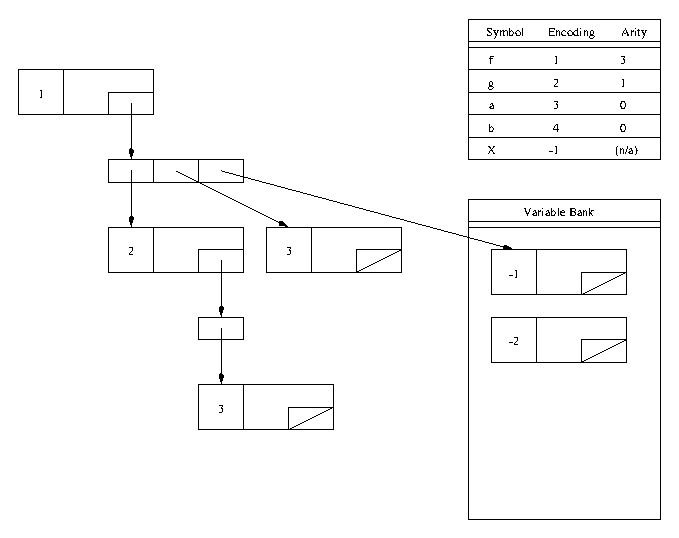
\epsfig{file=unshared_terms.eps}}
    \caption{Representation for the term \texttt{f(g(a),a,X)}}
    \label{fig:terms:unshared}
  \end{center}
\end{figure}

A cell for each term node contains information about the function
symbol, and a pointer to an array of argument terms. It also contains
additional information about the term and slots used only for the
implementation of functionality of shared terms. A term cell is
realized as the following C language \texttt{struct} (only elements
necessary for unshared terms are shown here, see
section~\ref{sec:terms:banks} for a more complete picture):

\small
\begin{verbatim}
typedef struct termcell
{
   TermProperties   flags;   /* Like basic, lhs, top */
   FunCode          f_code;  /* Top symbol of term */
   int              arity;   /* Redundant, but saves handing around
                                the signature all the time */
   struct termcell* *args;   /* Pointer to array of arguments */
   struct termcell* binding; /* For variable bindings, potentially
                                for temporary rewrites */
   ...
}TermCell, *Term_p, **TermRef;
\end{verbatim}
\normalsize

\begin{description}
\item[\textmd{\texttt{flags}}:] Stores special properties for term
  nodes. This feature is discussed in the next section.
\item[\textmd{\texttt{f\_code}}:] The encoded function symbol or
  variable.
\item[\textmd{\texttt{arity}}:] The number of principal subterms of
  this term cell. If this is 0, the \texttt{args} element should
  contain \texttt{NULL}, otherwise it should point to an memory block
  of size \texttt{arity*sizeof(Term\_p)} that is interpreted as an
  array of \texttt{Term\_p} pointers.
\item[\textmd{\texttt{args}}:] Pointer to the array or argumens.
\item[\textmd{\texttt{binding}}:] If this pointer is not
  \texttt{NULL}, it points to another term, that can be used instead
  of the current term cell (and corresponding term). This feature is
  mainly intended for the instantiation of variables, but can also be
  used if you want to modify a term temporarily. Most functions on
  terms can be told to follow or ignore bindings.
\end{description}


\subsubsection{Term Properties}

Term properties are stored in individual bits of the \texttt{flags}
field. The relevant data type, \texttt{TermProperties}, is defined as
an enumeration type in \texttt{cte\_terms.h}\footnote{According to the
  ANSI C standard, enumeration values are compatible with \texttt{int}
  values, i.e. they have at least 32 bits. Thus, 32 distinct
  properties can be assigned to each term.}. Only a few values are
predefined by the library, other values can be defined by the user.

\small
\begin{verbatim}
typedef enum 
{
   TPIgnoreProps = 0, /* For masking properties out */
   TPMaximal     = 1, /* Maximal term == Left hand side */
   TPTopPos      = 2, /* This cell is a entry point */
   TPBasicPos    = 4, /* Basic position on this term */
   TPPredPos     = 8, /* This is an previous predicate position
                         morphed into a term */
   TPOpFlag      = 256,/* For internal use */
   TPOutputFlag  = 512 /* Has this term already been printed? */
}TermProperties;
\end{verbatim}
\normalsize

As properties are bit-valued, they can be combined with the binary
\emph{or}-operator ('\texttt{|}').  Properties are manipulated by
three functions (realised as C preprocessor macros):

\begin{verbatim}
MACRO void TermSetProp(Term_p term, TermProperties prop)
\end{verbatim}
\begin{quote}
  Set the given properties in the term.
\end{quote}

\begin{verbatim}
MACRO void TermDelProp(Term_p term, TermProperties prop)
\end{verbatim}
\begin{quote}
  Delete the given properties in the term.
\end{quote}
\begin{verbatim}
MACRO bool TermQueryProp(Term_p term, TermProperties prop)
\end{verbatim}
\begin{quote}
  Query the given properties. The result is true if all the queried
  properties are set in the term.
\end{quote}


\subsection{Term Banks}
\label{sec:terms:banks}

Term banks are structures for building shared terms. 




%%% Local Variables: 
%%% mode: latex
%%% TeX-master: "clib"
%%% End: 


\end{document}

%%% Local Variables: 
%%% mode: latex
%%% TeX-master: t
%%% End: 
